
\documentclass[a4paper,11pt]{article}

\usepackage[T1]{fontenc}
\usepackage[utf8]{inputenc}
\usepackage{graphicx}
\usepackage{xcolor}

\renewcommand\familydefault{\sfdefault}
\usepackage{tgheros}
\usepackage[defaultmono]{droidmono}

\usepackage{amsmath,amssymb,amsthm,textcomp}
\usepackage{enumerate}
\usepackage{multicol}
\usepackage{tikz}

\usepackage{geometry}
\geometry{total={210mm,297mm},
left=25mm,right=25mm,%
bindingoffset=0mm, top=20mm,bottom=20mm}


\linespread{1.3}

\newcommand{\linia}{\rule{\linewidth}{0.5pt}}

% custom theorems if needed
\newtheoremstyle{mytheor}
    {1ex}{1ex}{\normalfont}{0pt}{\scshape}{.}{1ex}
    {{\thmname{#1 }}{\thmnumber{#2}}{\thmnote{ (#3)}}}

\theoremstyle{mytheor}
\newtheorem{defi}{Definition}

% my own titles
\makeatletter
\renewcommand{\maketitle}{
\begin{center}
\vspace{2ex}
{\huge \textsc{\@title}}
\vspace{1ex}
\\
\linia\\
\@author \hfill \@date
\vspace{4ex}
\end{center}
}
\makeatother
%%%

% custom footers and headers
\usepackage{fancyhdr}
\pagestyle{fancy}
\lhead{}
\chead{}
\rhead{}
\lfoot{SimTools Project 1}
\cfoot{}
\rfoot{Page \thepage}
\renewcommand{\headrulewidth}{0pt}
\renewcommand{\footrulewidth}{0pt}
%

% code listing settings
\usepackage{listings}
\lstset{
    language=Python,
    basicstyle=\ttfamily\small,
    aboveskip={1.0\baselineskip},
    belowskip={1.0\baselineskip},
    columns=fixed,
    extendedchars=true,
    breaklines=true,
    tabsize=4,
    prebreak=\raisebox{0ex}[0ex][0ex]{\ensuremath{\hookleftarrow}},
    frame=lines,
    showtabs=false,
    showspaces=false,
    showstringspaces=false,
    keywordstyle=\color[rgb]{0.627,0.126,0.941},
    commentstyle=\color[rgb]{0.133,0.545,0.133},
    stringstyle=\color[rgb]{01,0,0},
    numbers=left,
    numberstyle=\small,
    stepnumber=1,
    numbersep=10pt,
    captionpos=t,
    escapeinside={\%*}{*)}
}

%%%----------%%%----------%%%----------%%%----------%%%

\begin{document}

\title{Simulation Tools FMNN05 \\Project 1}

\author{Nils Fagerberg, Daniel Odenbrand, Felicia Seemann and Linus Jangland}

\date{\today}

\maketitle

\section*{Background}
As a part of the course Simulation Tools, FMNN05, at LTH there are three projects related to simulating solutions of differential equations using the tools Assimulo/Sundials, Dymola/Modelica and the programming language Python. 

Every project is divided into smaller tasks. We will present each task followed by its results one by one. This is the report for project 1.

\section{The elastic pendulum problem}
Task 1 consisted of a model for an elastic pendulum given by the following ODE
\begin{align}
& \dot{y_1} = y_3 \\
& \dot{y_2} = y_4 \\
& \dot{y_3} = -y_1 \cdot \lambda (y_1, y_2) \\
& \dot{y_4} = -y_1 \cdot \lambda (y_1, y_2)  - 1
\end{align}

where $\lambda (y_1, y_2) = k \frac{\sqrt{y_1^2 + y_2^2} - 1}{\sqrt{y_1^2 + y_2^2}}$. This corresponds to a mathematical pendulum where the bar is replaced by a linear spring with spring constant $k$. The mass-, nominal pendulum length and gravitational constant are taken to be one.

The task is to set up this problem in Python and solve it using Assimulo.

\subsection*{Solution}
The code for task 1 can be viewed below:

\begin{lstlisting}[caption=Script for solving Task 1]
#lambda(y1, y2, k)
def lambda_func(y1, y2, k = 1):
    return k*(np.sqrt(y1**2 + y2**2) - 1)/np.sqrt(y1**2 + y2**2)

#the right hand side of our problem
def rhs(t, y):
    return np.array([y[2], y[3], -y[0]*lambda_func(y[0], y[1]), -y[1]*lambda_func(y[0], y[1]) - 1])

#initial values. y[0] = x-position, y[1] = y-position, y[2] = x-velocity, y[3] = y-velocity
y0 = np.array([1.0, 0.0, 0.0, -1.0])
t0 = 0.0

#Assimulo stuff
model = Explicit_Problem(rhs, y0, t0)
model.name = 'Task 1'
sim = CVode(model)
sim.maxord = 7
tfinal = 100.0
#simulation. Store result in t and y
t, y = sim.simulate(tfinal)

#Create plots. Three figures are created: one containing positional values as a function of time, one with velocities as a function of time and the last traces the pendulum's movement (x and y coordinates in cartesian coordinate)
fig, ax = plt.subplots()
ax.plot(t, y[:, 0], label='x-pos')
ax.plot(t, y[:, 1], label='y-pos')
legend = ax.legend(loc='upper center', shadow=True)

plt.figure(1)
fig2, ax2 = plt.subplots()
ax2.plot(t, y[:, 2], label='x-vel')
ax2.plot(t, y[:, 3], label='y-vel')
legend = ax2.legend(loc='upper center', shadow=True)

plt.figure(1)
fig3, ax3 = plt.subplots()
ax3.plot(y[:, 0], y[:, 1], label='displacement')
legend = ax3.legend(loc='upper center', shadow=True)

# Now add the legend with some customizations.
plt.show()
\end{lstlisting}

We use the solver CVode.

%\newpage
\subsection*{Results}
Below some resulting plots of our implementation can be seen. All plots are in the time-interval 0 to 20 and the initial values are all zeros except for the $x$ which is set to 1 without elongations since the pendulum length is 1.

\begin{figure}[!h]
\centering
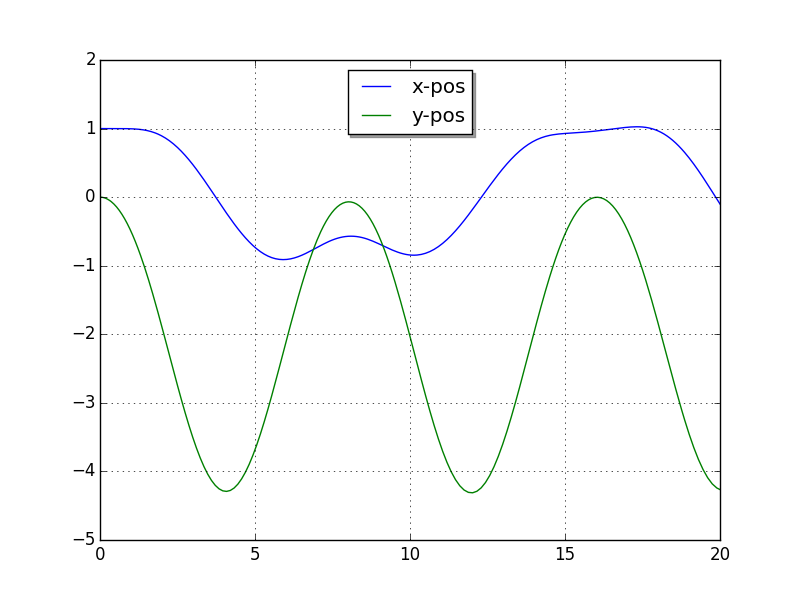
\includegraphics[scale=0.5]{task1_k075_1.png}
\caption{x and y positions as functions of time, with $k = 0.75$}
\label{1k075}
\end{figure}

\begin{figure}[!h]
\centering
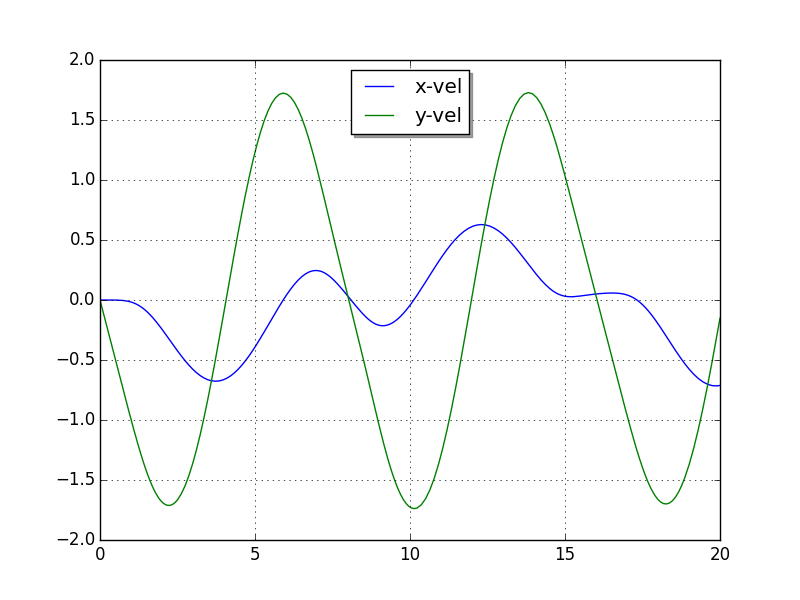
\includegraphics[scale=0.5]{task1_k075_2.png}
\caption{velocities in x- and y-directions as functions of time, with $k = 0.75$}
\label{2k075}
\end{figure}

\begin{figure}[!h]
\centering
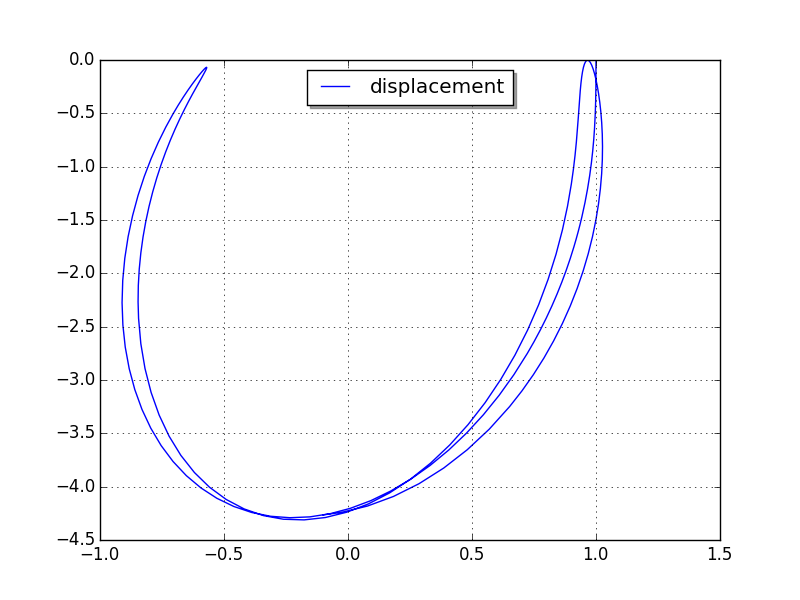
\includegraphics[scale=0.5]{task1_k075_3.png}
\caption{tracings of the pendulum trajectory for $k = 0.75$}
\label{3k075}
\end{figure}

In figures \ref{1k075}, \ref{2k075} and \ref{3k075} we have used the spring constant $k = 0.75$ which is very elastic as seen specifically in figure \ref{3k075} where the pendulum does an irregular motion. The y-position varies between 0 and about -4 and the x-position varies between 1 and -1 according to figure \ref{1k075}. Also the y-velocity is more regular than the x-velocity, as seen in figure \ref{2k075}.

\begin{figure}[!h]
\centering
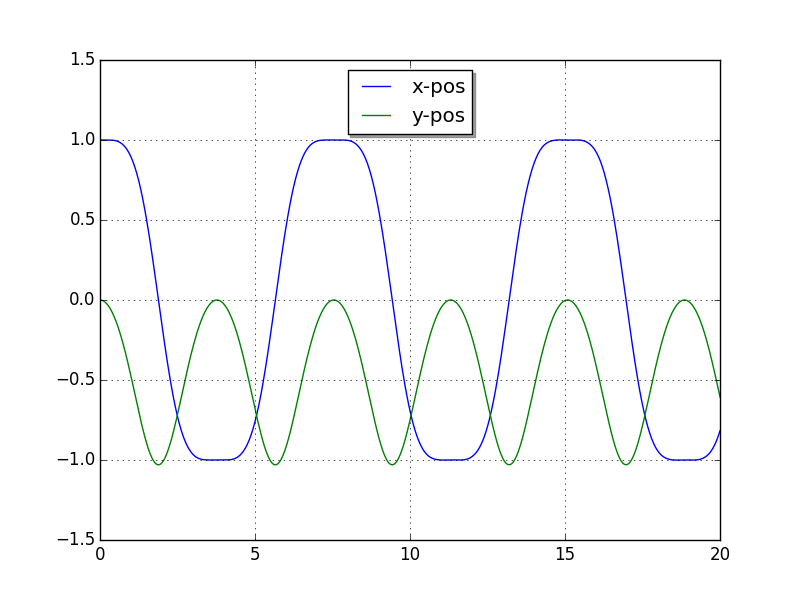
\includegraphics[scale=0.5]{task1_k100_1.png}
\caption{x and y positions as functions of time, with $k = 100$}
\label{1k100}
\end{figure}

\begin{figure}[!h]
\centering
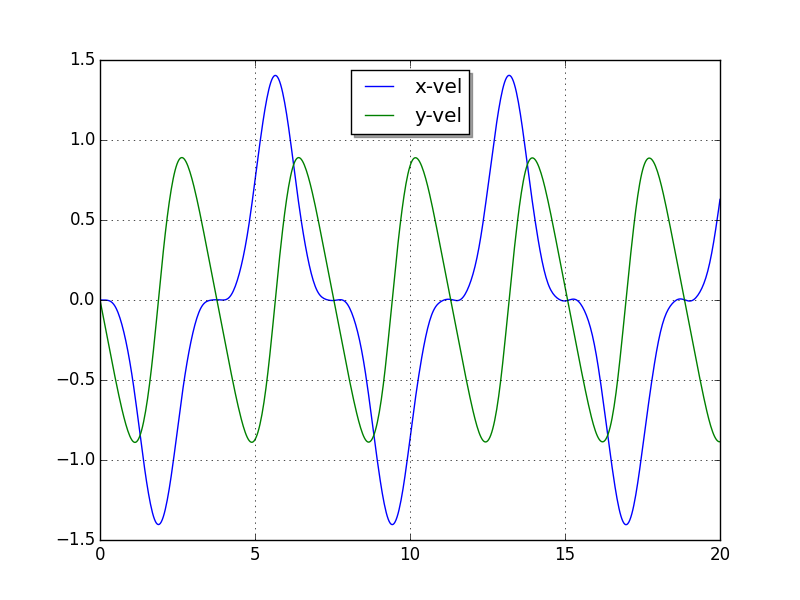
\includegraphics[scale=0.5]{task1_k100_2.png}
\caption{velocities in x- and y-directions as functions of time, with $k = 100$}
\label{2k100}
\end{figure}

\begin{figure}[!h]
\centering
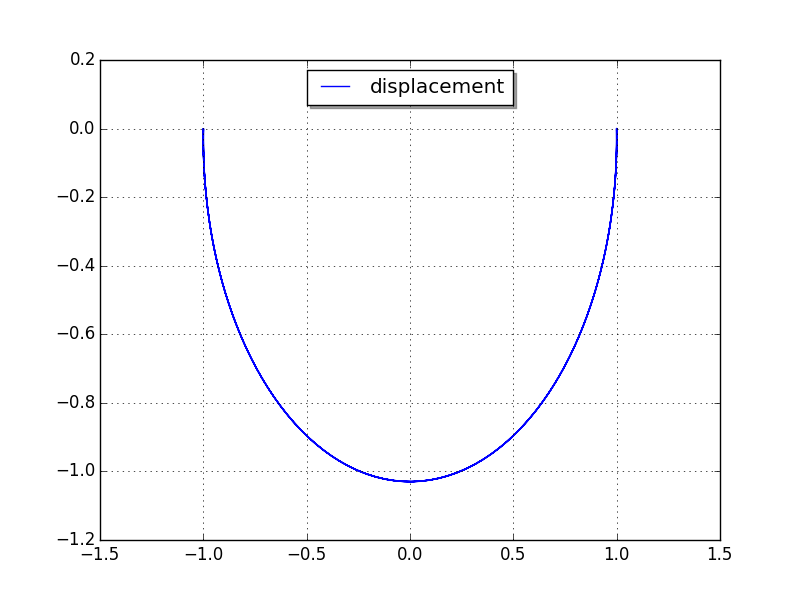
\includegraphics[scale=0.5]{task1_k100_3.png}
\caption{tracings of the pendulum trajectory for $k = 100$}
\label{3k100}
\end{figure}

In contrast, figures \ref{1k100}, \ref{2k100} and \ref{3k100} display results of a more stiff pendulum ($k = 100$). As is visible in figure \ref{3k100}, the pendulum trajectory is uniform and rather unexciting. The positional values and velocities are very periodic as you would expect from e.g. a grandfather clock.

\begin{figure}[!h]
\centering
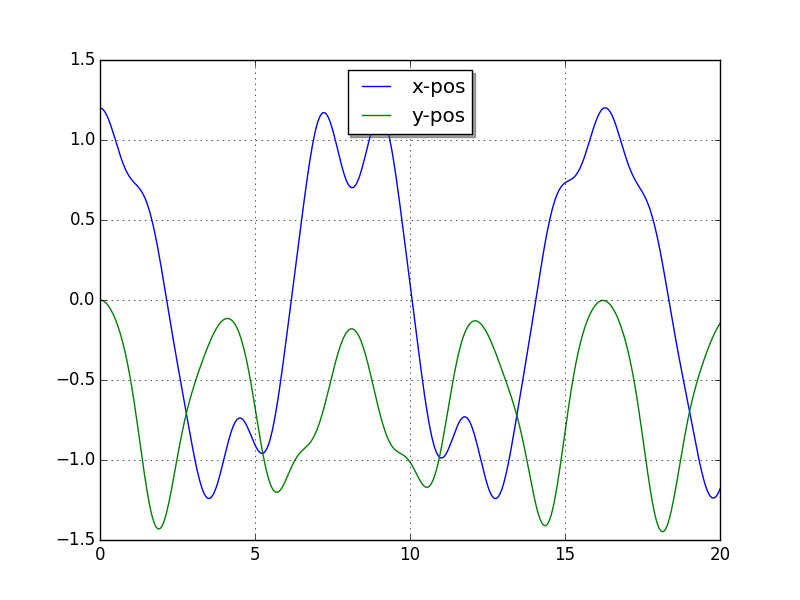
\includegraphics[scale=0.5]{task1_k10_utdrag12_1.png}
\caption{x and y positions as functions of time, with $k = 10$}
\label{1k10}
\end{figure}

\begin{figure}[!h]
\centering
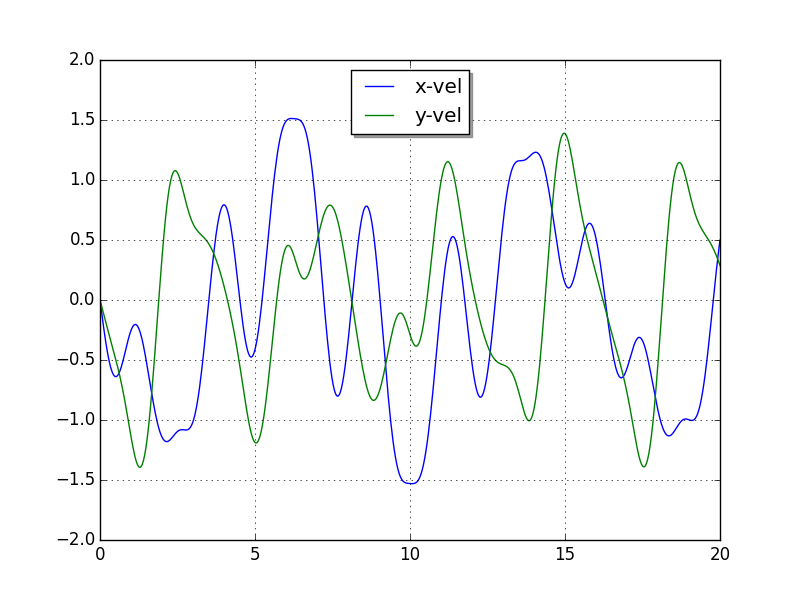
\includegraphics[scale=0.5]{task1_k10_utdrag12_2.png}
\caption{velocities in x- and y-directions as functions of time, with $k = 10$}
\label{2k10}
\end{figure}

\begin{figure}[!h]
\centering
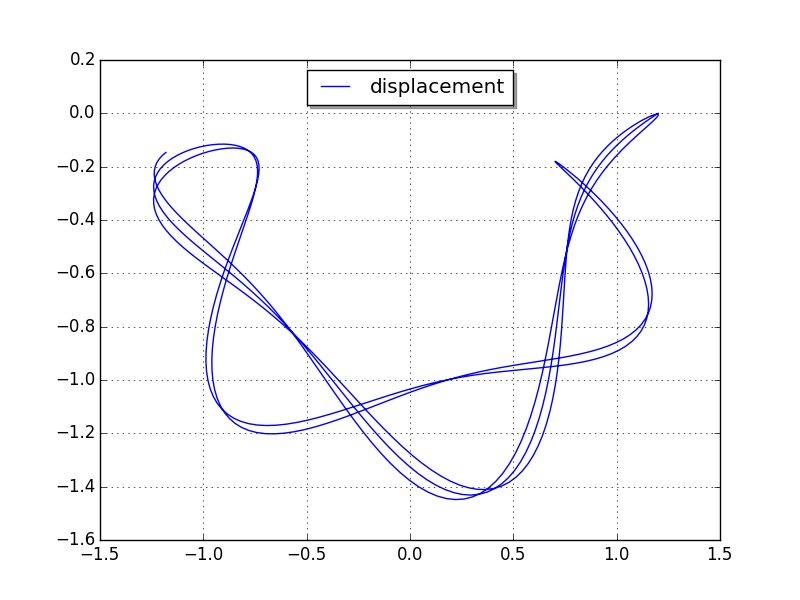
\includegraphics[scale=0.5]{task1_k10_utdrag12_3.png}
\caption{tracings of the pendulum trajectory for $k = 10$}
\label{3k10}
\end{figure}

To obtain an oscillation around the trajectory of a stiff pendulum we can start with an elongation of the spring (we used $x = 1.2$ as initial value) which would result in the pendulum contracting. Some plots of this are visible in figures \ref{1k10}, \ref{2k10} and \ref{3k10}. We can also see that the y-position and y-velocity values are a bit more irregular.

\subsection*{Discussion}
We can see that the spring is very elastic in figure \ref{3k075} since the pendulum is stretched out about 4 times its original size. Despite this, we observe a very low disturbance in the y-position and y-velocity's periodicities. This is due to the force from the spring being much lower than the gravitational force acting on the pendulum. The x-values, however are unaffected by gravity, resulting in a visible effect. This hypothesis is reinforced by the figures from the stiff pendulum, where $k = 100$, in which the x-values also become very periodic.

With a initial elongation of the spring we would expect the y-values to become more irregular since the spring is oscillating around its equilibrium.

\section{BDF3 and BDF4}
Our implementations of BDF-4 and BDF-3 can be seen in Listings \ref{BDF3} and \ref{BDF4}.

\begin{lstlisting}[caption = Python implementation of BDF3, label = BDF3]
    def step_BDF3(self,T,Y):
        """
        BDF-3 with fsolve
        """
        alpha = [11/6, -18/6, 9/6, -2/6]
        return self.step_BDFn(T, Y, 3, alpha)
\end{lstlisting}

\begin{lstlisting}[caption = Python implementation of BDF4, label = BDF4]
    def step_BDF4(self,T,Y):
        """
        BDF-4 with fsolve
        """
        alpha = [25/12, -48/12, 36/12, -16/12, 3/12]
        return self.step_BDFn(T, Y, 4, alpha)
\end{lstlisting}

Both of these use the function BDFn, which can be seen in Listing \ref{BDFn}.

\begin{lstlisting}[caption = Auxiliary function BDFn, label = BDFn]
    def step_BDFn(self, T, Y, n, alpha):
        """
        Performs a BDF step of order n
        """
        f = self.problem.rhs
        h = self.h
        # predictor
        t_np1 = T[0] + h
        y_np1_i = Y[0] # zero order predictor
        def g(y_np1):
            return alpha[0]*y_np1 + sum([alpha[i+1]*Y[i] for i in range(n)]) - h*f(t_np1, y_np1)
        y_np1 = so.fsolve(g, y_np1_i)
        return t_np1, y_np1
\end{lstlisting}

\section{Assimulo testing for various frequencies using a BDF solver}
%insert experiments with different methods

\section{Assimulo testing using CVode}
Now we repeat the experiments from task 3 using the solver CVode again. We also test the influence of ATOL, RTOL, MAXORD and the choice of discretization on the performance for the low and highly oscillating case.

\subsection*{Low oscillation}
Here we will test different parameters using $k = 10$ and the initial elongation $x = 1.2$, for a low oscillation.

\subsubsection*{ATOL and RTOL}
%SKRIV NÅT VETTIGT om atol vs rtol 


Both of these options concern error tolerances and are therefore discussed together. Having a higher tolerance will allow the solver to take larger steps, thus making the solution look choppy, as seen in figure \ref{3k10at01}.

\begin{figure}[!h]
\centering
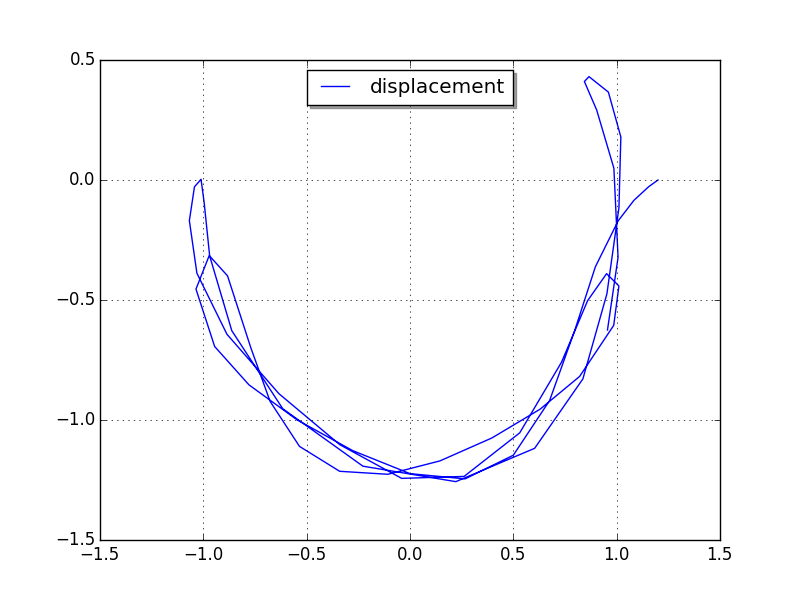
\includegraphics[scale=0.5]{task1_k10_utdrag12_atol01.png}
\caption{tracings of the pendulum trajectory for $k = 10$ with $atol = 1$}
\label{3k10at01}
\end{figure}

\begin{figure}[!h]
\centering
\includegraphics[scale=0.5]{task1_k10_utdrag12_rtol01.png}
\caption{tracings of the pendulum trajectory for $k = 10$ with $rtol = 1$}
\label{3k10rt01}
\end{figure}

\subsubsection*{MAXORD}
The maximum order of a method determines the number of past points that are used as reference for approximating the next value. A high order method will have the potential for taking larger steps at the cost of more computations per step. To ensure the same accuracy with a lower order method we must take smaller steps. For example running our code from task 1 using the order 1 takes 38501 steps, compared to the 536 steps taken using the default order (12).

\subsubsection*{Choice of discretization}
We compared both discretization using Adams method and the BDF method. Both methods generated a displacement-graph which were very much simular to each other. There are some differences in the number of steps and evaluation that both methods use, but the run-times are practically the same (Adams is slightly faster).

\subsection*{High oscillation}
Now  we test the different parameters' influence in the highly oscillating case, using $k = 50$ and initial elongation $x = 1.2$.

\subsubsection*{ATOL and RTOL}

%SKRIV NÅ VETTIGT

\begin{figure}[!h]
\centering
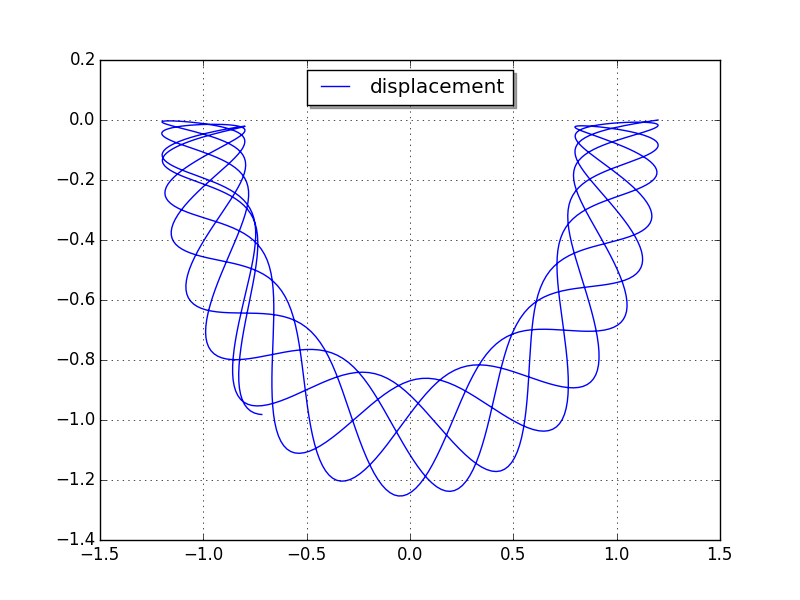
\includegraphics[scale=0.5]{task1_k50_utdrag12_default.png}
\caption{tracings of the pendulum trajectory for $k = 50$ with default a- and rtol}
\label{3k10at01}
\end{figure}

\begin{figure}[!h]
\centering
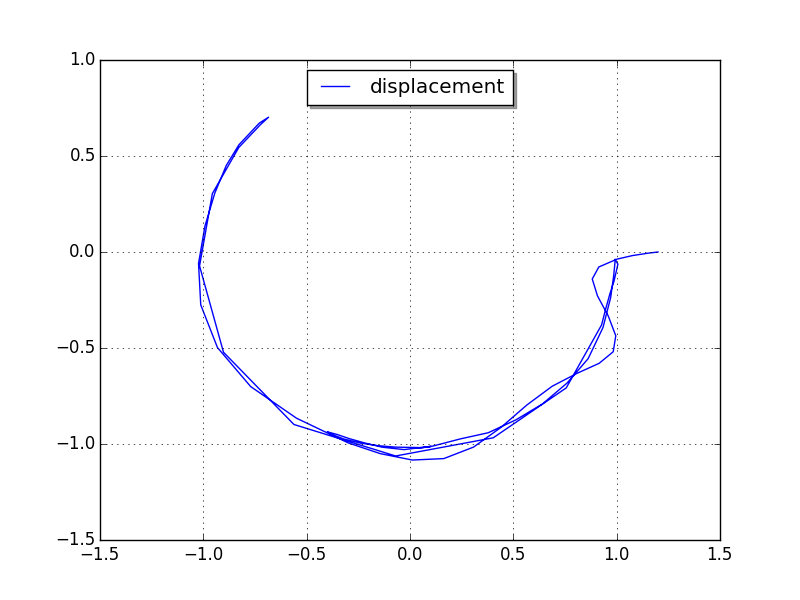
\includegraphics[scale=0.5]{task1_k50_utdrag12_atol01.png}
\caption{tracings of the pendulum trajectory for $k = 50$ with $rtol = 1$}
\label{3k10rt01}
\end{figure}

\begin{figure}[!h]
\centering
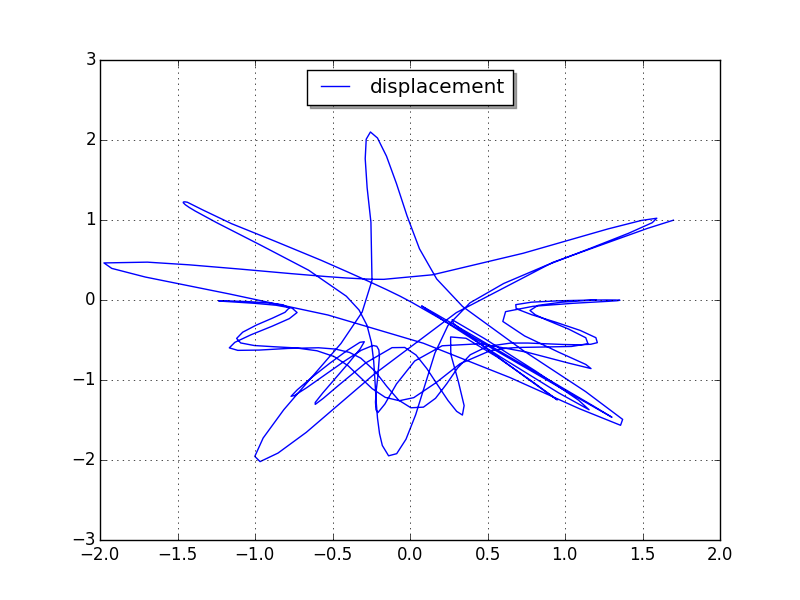
\includegraphics[scale=0.5]{task1_k50_utdrag12_rtol01.png}
\caption{tracings of the pendulum trajectory for $k = 50$ with $atol = 1$}
\label{3k10at01}
\end{figure}

\subsubsection*{MAXORD}
The maximum order still only affects the number of steps. The highly oscillating case originally takes more steps than the low oscillation (1100 steps), thus it makes sense that when using maximum order 1 we get about twice as many steps compared to the low oscillation case (76856 steps)

\subsubsection*{Choice of discretization}


\section{Comparison of Assimulo and Dymola}
In this section we will examine the possibilities to simulate the pendulum in Dymola. We will especially consider different integrators and compare them when run in Assimulo and in Dymola. The number of steps that the integrator uses gives us an idea of how large steps the method is taking, thus also how fast the method might be running. Though the actual time consumed in each step is in the function evaluations. Each step does a number of function evaluations, and if a method uses many evaluations it might be less efficient than a method with more steps but fewer evaluations. In the table below our results can be viewed:

\begin{table}
\begin{tabular}{|c|c|c|}
\hline
Method \textbackslash \, Program & Assimulo & Dymola  \\ \hline
\begin{tabular}{c}
\\
Explicit Euler \\ 
Dopri45 \\
CVode \\ 
Lsodar \\
\end{tabular}
& \begin{tabular}{c|c|c|c}
steps & calls & J-eval & nonlinear \\ \hline
2000 & 2000 & 0 & 0 \\ \hline
201 & 1208 & 0 & 0 \\ \hline
536 & 580 & 9 & 576 \\ \hline
362 & 747 & 0 & 0 
\end{tabular}
& \begin{tabular}{c|c|c|c}
steps & calls & J-eval & nonlinear \\ \hline
500 & 500 & 0 & 0 \\ \hline
193 & 1155 & 0 & 0 \\ \hline
544 & 585 & 10 & 581 \\ \hline
362 & 747 & 0 & 0 
\end{tabular}
\\ \hline
\end{tabular}
\caption{An overview of statistics for some methods present in both Assimulo and Dymola. Standard values used: $x = 1.2$, $k = 10$, $tol = 1e-6$ and $t=0..20$.}%A comparison of the number of steps taken, function calls, Jacobian evaluations and nonlinear iterations across a few methods present in both Assimulo and Dymola
\label{DymolaStatistics}
\end{table}

As seen in table \ref{DymolaStatistics} the Explicit Euler isn't affected by whether we're using Assimulo or Dymola (the step size is 4 times smaller by default in Assimulo). 

The Dopri45 integrator on the other hand differs a bit. To start with we can see that this integrator is a 4-5 step method since we have about 6 times as many function evaluations as steps (each step samples the right-hand side at 5 points, the 4th in two distinct ways). The deviations from the multiplicity are as a result of failed steps where we had to do another evaluation with some changes to succeed. For this method Dymola is a bit more efficient (fewer steps), compared to Assimulo.

Looking at the CVode integrator we can see that, compared to Dopri45, we have much fewer function evaluations. This is as a result of CVode being a one-step method (thus having almost the same amount of function calls as steps). The price we pay for having a one-step method on the other hand is the number of Jacobian evaluations and number of non-linear iterations. Our theory is that steps will more often fail when using a one-step method than when using a multi-step method. This time though Assimulo is more efficient than Dymola.

The last method considered is Lsodar. This seems to be a 2-step method and this time we do not get punished by having to take new Jacobian evaluations, as with CVode. The number of function calls surpasses the number used in CVode though. Using this integrator we have no difference in number of steps and function calls in Assimulo and Dymola.

On a particular machine we had the same CPU-time for CVode and Lsodar so we can compare the cost for Jacobian evaluations to function evaluations. We have (in Dymola) $747-585=162$ function evaluations more for Lsodar than CVode. This is compensated by 10 Jacobian evaluations, so we can assume that a Jacobian evaluation is about 16 times as costly as a normal function evaluation for this problem. Also the only conclusion we can draw about recommending an integrator for this problem is that Dopri45 is a bit slower than CVode and Lsodar and that Explicit Euler gives a really bad solution. Thus using either CVode or Lsodar seems reasonable.

\section{Discussion}

%WE DID THIS
%H*R LÄG IN E NTABEL OM MED CAPTIONS TYP ALLA PARMATTERRA RO SÅNT

\end{document}
